\documentclass{fsinewsletter}

\SetInfoprof{Ostermann}
\SetMatheprof{Dorn}
\SetMonth{Wintersemester}
\SetAuflage{1}
\SetJahr{2015}

\calvintrue %% comment für blank bilder
%\calvinfalse %% uncomment für blank bilder

\begin{document}

%%%% Titelseite
\thispagestyle{empty}
{\sf \number\auflage. Ausgabe \hfill Tübingen, 
%Wintersemester 2015/2016}
\Month\space \number\jahr}\\
\vspace{5cm}

%\rule[2mm]{\textwidth}{.2cm}\\

\includegraphics[width=\textwidth]{logos/fsi-log-logo}

%\rule{\textwidth}{0.2cm}\\
%{\sf \number\auflage. Auf\/lage \hfill Tübingen, \Month\space \number\jahr}\\

%\vspace*{2cm}
\begin{center}
%\oldbaselineskp=\baselineskip
%\baselineskip 45pt
%
%\Huge \name\\[2cm]
%
%
%\LARGE \Month \space \number\jahr
%\\
%
%\baselineskip=\oldbaselineskp
\vfill
%
\includegraphics[width=\textwidth]{logos/fsilogo}
%\uni H \rm ~~~ \raisebox{18pt}{\Huge Universität Tübingen}\\[2cm]
\end{center}
\eject


%%%% Inhaltsverzeichniss
\tableofcontents
\newpage

%%%%%%%%%%%%%%%%%%%%%%%%%%%%%%%%%%%%%%%%%%%%%%%%%%%%%%%%%%%%%%%%%%%%%%%%%%%%%
%%% Inhalt hier eintragen
%%%%%%%%%%%%%%%%%%%%%%%%%%%%%%%%%%%%%%%%%%%%%%%%%%%%%%%%%%%%%%%%%%%%%%%%%%%%%

%%%% Vorwort
\section{Vorwort}
\Large
Liebe Lesende,\\
\\
\normalsize
hiermit veröffentlichen wir die erste Ausgabe unseres \nameit. Alle, die nun ein Exemplar des \nameit \space in der Hand halten: schön, dass ihr Interesse an unserer und eurer Zeitschrift habt! 

Wir haben letztes Semester wie immer mit zahlreichen Erstsemesterveranstaltungen begonnen. Mit über 300 neuen Erstsemestern gab es wieder einiges zu tun.
Neben unseren klassischen Erstsemesterveranstaltungen konnten wir dieses Jahr unser Programm wieder erweitern. Nachdem vor einem Jahr das gemeinsame Grillen auf dem Sand hinzu kam, konnten wir dieses Jahr zusätzlich noch einen Spieleabend, eine Party und eine Wanderung nach Bebenhausen veranstalten.

Während des Semesters konnten wir dieses Jahr dank eurer Hilfe wieder eines der bestbesuchten Clubhausfeste ausrichten. Dieses Semester haben wir gemeinsam mit der Fachschaft Psychologie beschlossen, ein Drittel des Gewinns an Refugio und das Aufnahmelager Sand Schwalbenweg zu spenden. Zusätzlich habt ihr circa \EUR{70} für diese Projekte auf dem Clubhausfest gespendet! 

Wir wünschen euch viel Spaß beim Lesen dieses \nameit \space und freuen uns auf euer Feedback!\\

\large
\textbf{Eure Fachschaft}
\normalsize
\newpage

%******************************************************
%%%% Neues aus der Fachschaft
%******************************************************
\section{Neues aus der Fachschaft}
%\lipsum[1-3]
%\newpage

\subsection{Erstsemesterveranstaltungen}
\textbf{Dieses Jahr durften wir wieder über 300 Erstsemester begrüßen. Durch die Hilfe zahlreicher Fachschaftsmitgliedern und weiteren Helfern konnten wir in diesem Semester unser Programm weiter ausbauen. Zusätzlich zu den seid Jahren stattfindenden Veranstaltungen konnten wir noch einen Spieleabend, eine Party und eine Wanderung organisieren.}
%
%\textbf{Grillen}

Unsere Veranstaltungen starteten dieses Jahr wieder am Nachmittag der Vorkursklausur. Zum Ausgleich organisierten wir ein gemeinsames Grillen für die Vorkursler auf dem Sand. Ungefähr 100 Erstsemester wurden dabei von uns begrillt, sodass die vorhandenen Sitzgelegenheiten fast nicht ausreichten. Zum Glück konnten wir uns weitere Bierbänke und -tische vom Lehrstuhl von Professor Zell ausleihen, wofür wir uns an dieser Stelle nochmals herzlichst bedanken möchten.

%\textbf{Frühstück und Sandführung}
Weiter ging es am Freitag vor dem eigentlichen Semesterstart mit einem gemeinsamen Frühstück. Ziel ist ein gemütliches Zusammensitzen bei dem die Studierenden höherer Semester ihre Erfahrungen weitergeben und Erstsemester alle möglichen Fragen stellen können. An den langen Frühstückstafeln haben die Erstsemester außerdem die Möglichkeit sich gegenseitig schon ein wenig kennenzulernen.\\
In Zusammenarbeit mit der Mensa Morgenstelle konnten wir wieder für reichlich Kaffee, Tee, Saft, Brötchen und Belag sorgen. Traditionell werden die Erstsemester hier auch gleich von der Fachschaft und dem Professor der Informatik I begrüßt. Anschließend haben wir wieder Führungen über den Campus Morgenstelle angeboten, damit die Erstsemester schon einige Tage vor Beginn des Studienalltags die Umgebung kennenlernen können.\\
Am Nachmittag wurden die einzelnen Studiengänge nochmals gesondert von einigen Professoren auf dem Sand begrüßt. Anschließend bestand für die Erstsemester die Möglichkeit sich einige Arbeitsbereiche des Instituts genauer anzuschauen. Dank der Mithilfe zahlreicher Professoren konnten an \todo{Anzahl der Stationen} Stationen die Arbeit der Lehrstühle begutachtet werden.
%
%\textbf{Kneipentour}
%
%\textbf{Stadtführung}
%
%\textbf{Spieleabend}

Zum ersten Mal veranstalteten wir in diesem Semester einen Spieleabend für die neuen Erstsemester. Dank der vielen Menschen, die eigene Spiele mitbringen, konnte aus einer Vielzahl von Spielen gewählt werden. In Kleingruppen wurde dann bis zum letzten Bus gespielt, gelacht und sich kennengelernt. Wir haben uns sehr über den großen Andrang und das positives Feedback gefreut und haben deshalb beschlossen, weitere Spieleabende auch außerhalb der Erstsemesterphase für alle Studierenden der Informatik anzubieten. Damit nicht jedes mal jeder Spiele mitbringen muss, haben wir eine kleine Auswahl angeschafft, die auch außerhalb von Spieleabenden von allen Informatikstudierenden benutzt werden darf
%\textbf{Party}

Neben den neuen Veranstaltungen organisierten wir auch zum ersten mal seit 2009 wieder einen Klassiker der Erstsemesterveranstaltungen, die Anfiparty. Hierbei waren alle Erstsemester herzlich eingeladen, auf ein Bier oder einen Glühwein in gemütlicher Runde auf den Sand zu kommen. Anschließend ging es dann gesammelt zur Semester Opening Party des Kuckucks in die Mensa Morgenstelle.
%wieder
%\textbf{Wanderung}

Eine weitere neue Veranstaltung in diesem Semester war einen gemeinsame Wanderung nach Bebenhausen, wo wir gemeinsam das mittelalterliche Kloster besichtigt haben.

%\textbf{Wochenende}
Den Abschluss der Erstsemesterveranstaltungen war das Anfiwochenende, welches wir mit den neuen Erstsemetern in einer Hütte im Umkreis von Tübingen verbringen.
Dieses Jahr ging die Reise nach Schachen, ein kleines Pfadfinderzentrum auf der schwäbischen Alp. Neben Aktionen wie Lagerfeuer, Nachtwanderung und Gruppenspielen im Freien war abends jede Menge Zeit sich beim gemütlichen Beisammensein kennenzulernen. 

Habt ihr coole Ideen, was wir noch an Veranstaltungen anbieten könnten? Oder habt ihr sogar Lust zu helfen? Dann kommt doch mal zu einer unserer Sitzungen\footnote{\url{http://www.fsi.uni-tuebingen.de/fachschaft/sitzung}} oder schreibt uns eine Mail\footnote{\email{fsi@fsi.uni-tuebingen.de}}.

\textbf{Helft uns dabei, die nächsten Erstsemesterveranstaltungen noch besser und noch größer zu machen!}

\subsection{Bundesfachschaftentagung Informatik}
Auch dieses Semester waren wieder Fachschaftsmitglieder auf der Konferenz der Informatik Fachschaften (KIF), der unserer Bundesfachschaftentagung. Auf der KIF kommen Fachschaften aus allen deutschsprachigen Ländern zusammen, um sich auszutauschen und Leute in verschiedene Gremien zu wählen.\\
In diesem Semester fand sie in vom 11.11.2015 bis zum 15.11.2015 in Bonn statt. Wir waren dort dieses mal mit drei Fachschaftlern vertreten.\\
Mittwoch Abend startete die KIF zunächst mit einem Anfangsplenum. Hier berichteten alle vertretenen Fachschaften und die von der KIF im vorhergegangenen Semester entsandten Vertreter kurz vor was seit der letzten KIF passiert ist. Anschließend wurden die Arbeitskreise, in denen die darauffolgenden Tagen gearbeitet und sich ausgetauscht wurde, vorgestellt.\\
Unsere Fachschaftler Erik Letzner, Philipp Zajac und Marc Weitz konnten in verschiedenen Arbeitskreisen wieder einige Ideen sammeln. Unter anderem enstand die Idee für diesen Newsletter.\\
Samstagabend begann schließlich das Abschlussplenum. Hier wurden die Ergebnisse der Arbeitskreise vorgestellt, neue Vetreter in verschiedene Gremien entsandt oder Alte bestätigt. Abschließend wurde noch eine Resolution versabschiedet, in der wir uns kritisch gegenüber der Novelierung des sogenannten Wissenschaftszeitvertragsgesetz äußern.\\
Mit diesem Gesetzesentwurf soll die Situation der zahlreichen Wissenschaftler verbessert werden, die immer wieder nur befristet angestellt werden. Auch wenn wir diese Intention begrüßen, gefährdet die aktuelle Fassung das Prinzip der studentischen Hilfskräfte. Mit der beschlossenen Resolution fordern wir den Gesetzgeber auf an dieser Stelle noch einmal nachzubessern.



\vfill
\subsection{Arbeitsräume auf dem Sand}
Nachdem auf dem Sand trotz unseres Protests die zwei Poolräume C111 und F121 geschlossen wurden und damit sich die Anzahl der studentischen Arbeitsräume immer weiter verringert konnten wir mit unserer Unterschriftenaktion doch einige Verbesserungen erreichen. Zum einen haben wir die Zusage bekommen, dass Studierende die Seminarräume außerhalb der Belegungszeiten zum Lernen und Arbeiten nutzen können. Hierzu haben wir für euch eine Übersicht der dauerhaften Belegungen erstellt. Die Raumbelegung ist auch an unserem Aushang vor dem Fachschaftszimmer und auf unserer Website\footnote{http://www.fsi.uni-tuebingen.de/studium/raumplaene} einsehbar.\\
Desweiteren wurde der studentische Arbeitsraum C119 mit zwei Rechnern und einem Drucker ausgestattet, sodass auch weiterhin das Drucken von Übungsblättern und Abgaben möglich ist.
Außerdem haben wir von der Fachbereichsleitung die Zusage bekommen, dass die Institutsbibliothek mit einem elektronischen Öffnungssystem versehen wird. Mit diesem wird es für alle Informatikstudierende möglich sein, auch außerhalb der Öffnungszeiten, in die Bibliothek zu kommen. Dort sollen zudem die Arbeitsplätze weiter ausgebaut werden, um den Wegfall der Poolräume zu kompensieren.

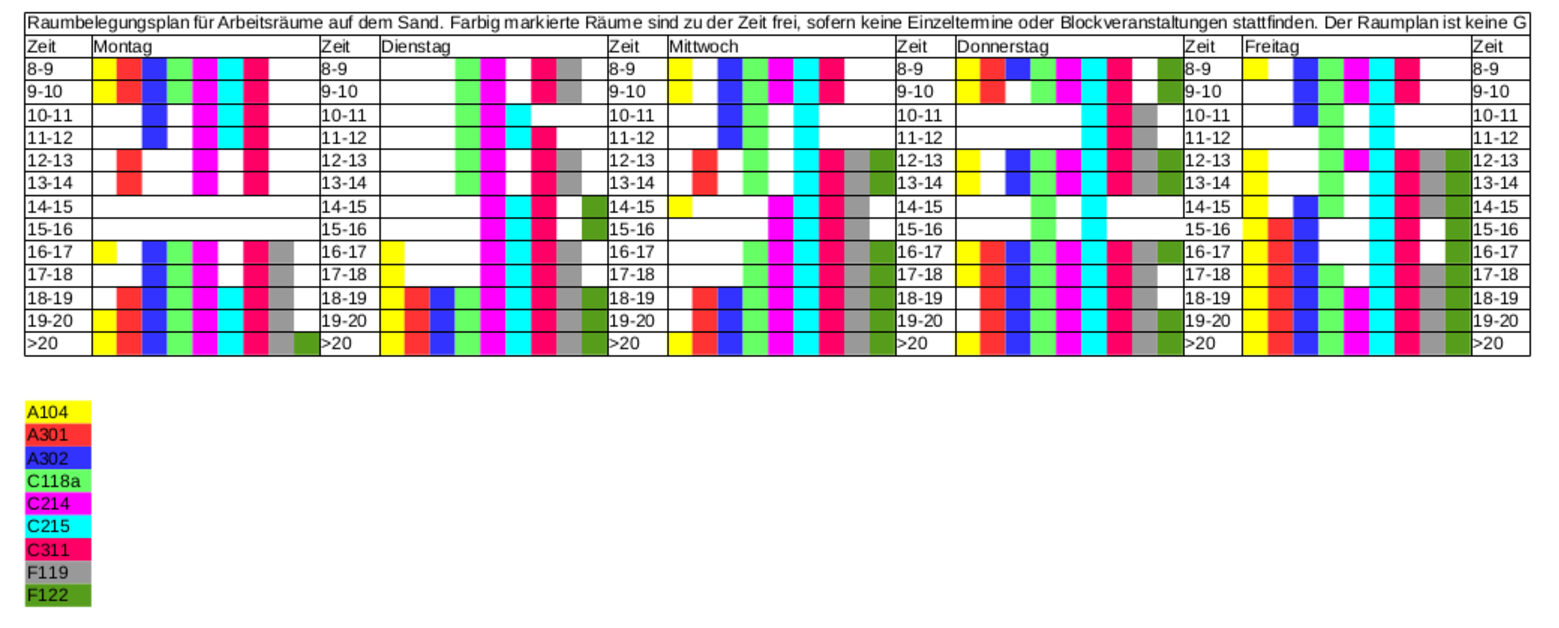
\includegraphics[width=\textwidth]{content/pictures/Raumplan.pdf}
\newpage

\subsection{Studientag 2015}
Jedes Jahr veranstaltet die Universität Tübingen den sogenannten Studientag. An diesem Tag können sich Schülerinnen und Schüler aus ganz Baden-Württemberg über die Studiengänge der Universität Tübingen informieren.\\
Wir waren selbstverständlich auch vertreten und konnten den Schülerinnen und Schülern zahlreiche Fragen vor allem auch aus unserer Sicht als Studierende beantworten.\\
Unsere beiden Stände auf der Morgenstelle mit den Studiengängen Informatik, Bioinformatik, Medieninformatik, Medizininformatik und Kognitionswissenschaft und in der Neuen Aula mit dem Studiengang Kognitionswissenschaft waren wie auch schon in den Vorjahren gut besucht.

\subsection{Clubhausfest}
Am 19.11.15 fand wieder das Clubhausfest der Fachschaften Informatik und Psychologie statt. Wie jedes Semester war unser Clubhausfest wieder sehr gut besucht.\\
Die Musikrichtungen waren in diesem Semester Drum'n'Base von Emernamin im kleinen Raum und die besten Hits der 2000er von Lousy Nova im großen Raum. Ergänzt wurden die beiden DJs von einem Auftritt von Professor Dr. Martin Butz, welcher eine eigene Playlist mitbrachte und auflegte.\\
Auch an der Bar waren zahlreiche Professoren vertreten. Die Professoren Bringmann und Zell wie Dr. Britta Dorn sorgten für den ausreichen Biernachschub für die Gäste.


\subsection{Spieleabend}
Nachdem großen Erfolg unseres Spieleabends für die diesjährigen Erstsemester haben wir beschlossen mehr oder wenig regelmäßig Spieleabende für alle Informatikstudierende anzubieten. Damit nicht jedes mal jeder alle seine Spiele mitbringen muss, haben wir einige Spiele angeschafft, die auch außerhalb der Spieleabende benutzt werden können. Solltet ihr auf dem Sand einmal Lust haben, eine Lernpause zu machen, schaut doch einfach mal in unserem Fachschaftszimmer vorbei und leiht euch ein Spiel aus.\\
Der letzte Spieleabend fand am 25.11.2015 statt und war wieder gut besucht. Bei kostenlosen Getränken und ausreichend Knabberzeug wurde wieder bis zum letzten Bus gespielt.\\
Auch im nächsten Semester wollen wir wieder Spieleabend für euch anbieten. Der nächste Termin steht noch nicht fest, wird aber rechtzeitig auf unserer Website\footnote{\url{www.fsi.uni-tuebingen.de}} und auf der Mailingliste info-studium bekannt gegeben.

\subsection{Prüfungszeiträume Kognitionswissenschaft}
Im Fachbereich Psychologie kam Ende 2015 der Vorschlag auf die Prüfungszeiträume dort neu zu gestalten. Was wieder einmal nicht bedacht wurde, war, dass dies auch den Studiengang Kognitionswissenschaft betrifft. Gemeinsam mit der Fachschaft Psychologie organisierten wir deshalb eine Umfrage, welches System bevorzugt wird. Die Ergebnisse dieser Umfrage werden wir auch in die nächste Studienkommisionssitzung Kognitionswissenschaft tragen und versuchen, eure Meinung dort durchzusetzen.
Gleichzeitig wird auch die Fachschaft Psychologie die Ergebnisse der Befragung zusammen mit den Ergebnissen der Befragung der Psychologiestudierenden in der Studienkommision Psychologie vertreten, welche bereits am 20.01. stattfindet. 

\subsection{Busverbindung Sand Morgenstelle}

\newpage
%******************************************************
%%%% Neues aus den Gremien
%******************************************************
\section{Neues aus den Gremien}

%\subsection{Studienkommisionen}

\subsection{Studierendenrat / FSRVV}
%Hochschulpolitik
Neben der Benennung von Vertretern für verschiedene Senatskommissionen und weitere Gremien und der finanziellen Unterstützung verschiedener Projekte gab es dieses Semester auch eine Aktion des StuRa und der FSRVV von der ihr wahrscheinlich etwas mitbekommen habt.\\
In den Mensen wurden Flyer verteilt, um auf die problematische Flyerpolitik des Studierendenwerkes als Mensaleitung aufmerksam zu machen. Die Regelungen der Mensa waren schon immer einschränkend (höchstens 5 Flyer gleichzeitig), als diese Regelung dann auf höchstens 2 Flyer beschränkt wurde, begann die Protestaktion. Eigentliches Ziel war, dass die Grenze grundsätzlich aufgehoben wird. Erreicht wurde zumindest, dass das StuWe die 5-Flyer-Regelung wieder eingeführt hat und sich auch wieder dran hält. Weitere Verbesserungen sollen im Gespräch erreicht werden.


\subsection{Fakultätsrat}
\todo{@Jonas3 Text schreiben}

\newpage
%******************************************************
%%%% Neues aus dem Institut
%******************************************************
\section{Neues aus dem Institut}

\subsection{Neue Professoren}
%An dieser Stelle möchten wir euch immer wieder die neuen Professoren hier am Institut vorstellen.
\todo{@Marc Luxburg ne Mail schreiben}
\Large \textbf{Ulrike von Luxburg}\\
\large Lehrstuhl für Theorie des Maschinellen Lernens\\
\normalsize

\begin{minipage}[h]{0.65\textwidth}
	\textbf{Kaffe oder Tee?}\\
	\\
	\textbf{Du oder Sie?}\\
	\\
	\textbf{Bleistift oder Kugelschreiber?}\\
	\\
	\textbf{Compilersprachen oder Scriptsprachen?}\\
	\\
	\textbf{Beamer oder Tafel?}\\
	\\
	\textbf{Windows, Linux oder OS X?}\\
	\\
\end{minipage}
\begin{minipage}[h]{0.35\textwidth}
	
\includegraphics[width=\textwidth]{content/pictures/no-image.jpeg}
\end{minipage}


\textbf{Was führt Sie an die Uni Tübingen?}\todo{Längere Fragen überlegen}

\newpage
This is an empty page
\newpage
\section{Follow Up}
Wir hoffen, euch hat die erste Ausgabe des \nameit \space gefallen.

Dieses Jahr wollen wir weitere Ausgaben des \nameit \space herausbringen. Dazu benötigen wir eure Hilfe. Denn ohne Inhalt ist das \nameit \space schon ziemlich langweilig. Daher suchen wir interessierte Personen, die uns dabei helfen, tolle Inhalte für die nächsten Ausgaben des \nameit \space zu erstellen. Wir können uns dabei ziemlich viel vorstellen, das für andere interessant sein könnte oder einfach nur lustig und cool ist:

\begin{itemize}
	\item Artikel zu interessanten Themen aus Informatik und Technik, aber auch zu Themen, die über den Tellerrand hinausgehen
	\item Erfahrungsberichte zum Studium, Auslandssemestern und anderen außergewöhnlichen Veranstaltungen
	\item Berichte über die aktuelle Arbeit in Fachgebieten oder kurze Artikel über eigene Seminar- und Abschlussarbeiten
	\item Selbstgezeichnete Comics, Rätsel, Bilder, Lieder, Gedichte, Rezepte, mathematische Beweise und was man sonst noch so abdrucken kann.
	\item Außerdem benötigt jede Ausgabe ein Titelbild.
\end{itemize}

Wenn ihr jetzt Lust bekommen habt mitzumachen, schickt eure Ideen und sonstigen Fragen an \email{fsi-log@fsi.uni-tuebingen.de} oder schaut bei einer Fachschaftssitzung vorbei. Wir freuen uns über eure Beiträge und werden dann zusammen mit euch schauen, was das nächste \nameit \space enthalten wird.\\

\large
\textbf{Eure Fachschaft}
\normalsize

\newpage
%******************************************************
%%%% Impressum und Rückseite
%******************************************************
\section{Impressum}
\nameit \space \space Januar 2016 - Zeitschrift der Studierenden des Fachbereiches Informatik der Eberhard Karls Universität Tübingen

Die Redaktion tagt derzeit unregelmäßig. Die Termine werden auf \url{www.fsi.uni-tuebingen.de} bekannt  gegeben.  Das  \nameit \space ist  im  Web  unter \url{www.fsi.uni-tuebingen.de/fachschaft/log}\todo{Link vervollständigen} verfügbar.

Interessierte Mitarbeiter sind immer willkommen; 
siehe \url{www.fsi.uni-tuebingen.de/log/mitmachen}
.
Namentlich gekennzeichnete und anonyme Beiträge geben nicht unbedingt die Meinung der Fachschaft wieder. Alle Rechte, insbesondere das der Verfilmung, vorbehalten.

Redaktionsanschrift:
\nameit, Fachschaft Informatik, Sand 14 C125, 72076 Tübingen\\
Webseite \url{www.fsi.uni-tuebingen.de}\\
E-Mail:\email{fsi@fsi.uni-tuebingen.de}

Redaktionsschluss dieser Ausgabe:\\
10. Januar 2016\\
Drucklegung dieser Ausgabe:\\
11. Januar 2016

V.i.S.d.P.: Marc Weitz, Fachschaft Informatik, Sand 14 C125, 72076 Tübingen\\
Redaktion: Lea Buchweitz, Jan-Peter Hohloch, Marc Weitz\todo{auflisten}\\
Satz: Marc Weitz mit \LaTeX 

Vielen Dank an die Autorinnen und Autoren der einzelnen Artikel und alle anderen, die zur Fertigstellung dieses Heftes beigetragen haben.



%\section{Kontakt}
%Wurde mit unserem \name{} interesse an Mitarbeit, Lob oder Kritik
geweckt, so freuen wir uns über digitale Post an
\url{fsi@fsi.uni-tuebingen.de} oder einen Besuch in der Sitzung
\textit{Donnerstags, 18:30 Uhr, Sand 14 Raum A104} (ggf abweichend,
aktuelle Sitzungstermine unter \url{http://www.fsi.uni-tuebingen.de/}) 

Die aktuellen studentischen Mitglieder der Gremien finden sich unter
\url{http://www.fsi.uni-tuebingen.de/fachschaft/vertreter}. 

Viele Kontaktadressen der in diesem \name{} aufgeführten aktiven Fachschaftler
und Gremienmitglieder finden sich unter
\url{http://www.fsi.uni-tuebingen.de/fachschaft/telefonliste}.
\todo{Liste aktualisieren!}
%%% Local Variables:
%%% mode: latex
%%% TeX-master: "../fachschafts_news"
%%% End:

\newpage
\section{Nächste Termine}
\large \centering
\begin{tabular}{llll}
	Wann? & & Wo? & Was?\\
	\hline
	22.10.2016 	& 18 Uhr	& Sand 14 Raum 	& LAN-Party \\
				&			&				& Spieleabend \\
\end{tabular}


\end{document}